\documentclass[12pt]{article}

% Packages
\usepackage[top=3cm, bottom=2cm, left=2cm, right=2cm]{geometry} % To change the margins
\usepackage[brazilian]{babel} % To use portuguese

\bibliographystyle{abntex2-alf}  % ABNT style for BibTeX

\usepackage{caption} % To change the caption name
\captionsetup[figure]{name=Fig.} % Change the caption name
\usepackage{subcaption} % To use subfigures
\usepackage[utf8]{inputenc} % To use special characters
\usepackage[T1]{fontenc} % To use special characters
\usepackage{graphicx} % To include images
\usepackage{url} % To include URLs
\usepackage{float} % To use H in figures
\usepackage{indentfirst} % To indent the first paragraph
\usepackage{wrapfig} % To inline images
\usepackage{needspace}  % Add to preamble if not present
\usepackage{hyperref} % For internal links
\usepackage{subcaption} % For subfiguress

\usepackage{hyperref}
\hypersetup{
    colorlinks=true,
    linkcolor=blue,      % For internal links like figures
    citecolor=blue,      % For citation links
    filecolor=magenta,   % For file links
    urlcolor=blue        % For URLs
}


% Document info
\title{\textbf{Janela de Pixels}}
\author{Igor Sousa Santos}
\date{}

\begin{document}

\maketitle

\section{O Escopo}

\subsection{Apresentação}
Se você já permaneceu mais de algumas horas em um ambiente sem janelas, sabe o quão difícil é saber como está o céu la fora. Essa desconexão com o mundo externo traz consigo um desconforto persistente que é difícil de colocar em palavras. O projeto descrito aqui visa reduzir este desconforto usando a placa de desenvolvimento BitDogLab. A matriz de LEDs pulsa com cores que seguem as percepções sociais das cores do céu de acordo com o horário. O display exibe uma pequena ilustração que mostra o período do dia (sol, lua, estrelas). O leve pulsar dos LEDs também ajuda a induzir um efeito calmante.

\begin{figure}[H]
    \centering
    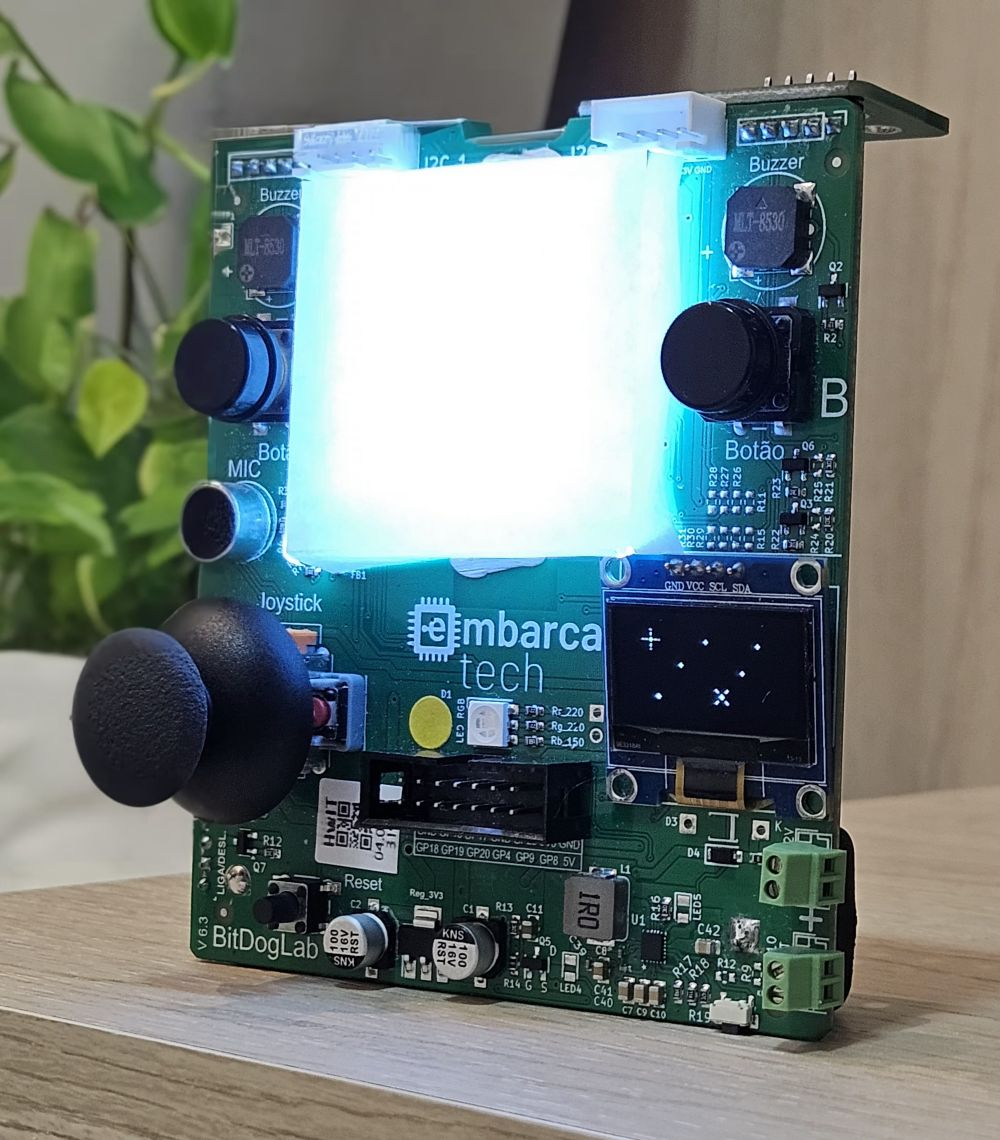
\includegraphics[width=0.4\textwidth]{resources/beautyshot.jpg}
    \caption{Janela de Pixels.}
    \label{fig:janeladepixels}
\end{figure}

\newpage

\subsection{O Objetivo}
\label{objetivo}
Os principais objetivos do projeto são:
\begin{enumerate}
    \item \textit{\textbf{Representar visualmente o céu externo.}}
    \item \textit{\textbf{Reduzir o desconforto de estar em um ambiente sem janelas.}}
    \item \textit{\textbf{Reduzir o stress.}}
\end{enumerate}

Nota-se aqui que os objetivos são difíceis de mensurar, com os efeitos no usuário sendo primariamente psicológicos. Embora seja possível avaliá-los por meio de estudos e questionários, as restrições de tempo e escopo do projeto impedem essa análise. Ainda assim, é essencial colocar as metas em termos concretos para que o projeto possa ser avaliado, logo podemos definir o principal objetivo como:

\begin{quote}
    \textbf{Exibir uma aproximação visual das cores do céu em um display de LED, que muda de acordo com a hora do dia.}
\end{quote}

A partir desse objetivo mais claro e concreto podemos começar a delinear os requisitos do projeto.

\subsection{Os Requisitos}
\label{requisitos}
Existem duas partes para os requisitos: aqueles do curso de capacitação a qual o projeto está inserido e os requisitos do cliente. Primeiramente veremos os requisitos do curso: 

\subsubsection{Requisitos do Curso}
\label{requisitoscurso}
\begin{itemize}
    \item Uso da placa de desenvolvimento BitDogLab.
    \item Restringir-se aos conceitos e tecnologias vistos no curso.
    \item Algum grau de inovação.
\end{itemize}

\subsubsection{Requisitos do Cliente}
Já para os requisitos do cliente, temos que primeiro definir os clientes em si: Um deles é o próprio desenvolvedor, que passa horas e horas escrevendo código em um quarto fechado com apenas uma pequena janela. O segundo cliente é a irmã do desenvolvedor que estuda em uma universidade sem janelas.

Partindo dessa definição dos solicitantes podemos então delinear seus requisitos. Lembrando que segundo (CUGNASCA C. E.)\cite{cugnasca} existem dois tipos principais de requisitos: Funcionais e Não Funcionais.
Começando com os requisitos \textbf{não funcionais} (menos específicos) temos:

\begin{itemize}
    \item Poder dizer de relance se está claro ou escuro do lado de fora.
    \item Implementação simples, sem alarmes ou mudanças bruscas de luminosidade que podem distrair os clientes.
    \item Simples de usar. Configuração e interação mínima. Ou seja, \textit{set it and forget it}.
    \item Mostrar cores visualmente atraentes.
    \item Mostrar desenhos bonitinhos na telinha.
\end{itemize}

A partir disso foram estabelecidos os \textbf{requisitos funcionais} (mais específicos):

\begin{itemize}
    \item Exibir cores de acordo com uma paleta escolhida pelos clientes na matriz de LEDs.
    \item A cor exibida deve mudar de horário de acordo com o passar do dia.
    \item A matriz de LEDs deve desligar durante o período noturno entre às 22:00 e 06:00 
    \item A cor exibida deve ter um efeito de modulação de brilho, não pode ser estática.
    \item O display deve exibir uma imagem representativa com o período do dia:
        \subitem Sol para o período entre às 06:00 e 18:00
        \subitem Lua para o período entre às 18:00 e 22:00
        \subitem Estrelas para o período entre às 22:00 e 06:00
    \item Botão de liga e desliga
    \item A matriz de LEDs deve ser ligada automaticamente às 06:00 para servir como um alarme luminoso.
    \item O horário da mudança das cores deve ser ajustado ao longo do ano, de acordo com o horário do nascer e pôr do sol.
    \item Pode funcionar usando uma fonte de energia cabeada, mas o uso da bateria interna seria um bom adicional. 
\end{itemize}

Um outro requisito opcional também foi definido pelos clientes:
\begin{itemize}
    \item A imagem no display deve indicar condiçoes climáticas:
    \subitem Adicionar pingos de chuva caso esteja nublado
    \subitem Adicionar nuvems caso esteja chuvendo
\end{itemize}

\subsection{Funcionamento}
Agora que temos os requisitos dos clientes, podemos descrever o funcionamento completo do projeto, considerando também as limitações de tempo do desenvolvedor.
Primeiramente é necessário que a placa BitDogLab tenha acesso ao horário atual, então usaremos o chip de rede da placa para se conectar a internet e adquirir o horário através de algum servidor ou endpoint. Aqui foi feita a primeira concessão ao desenvolvedor:
\paragraph{Problema:} 
Para se conectar à internet é necessário configurar o SSID e a senha de uma rede WiFi, no entanto a implementação de uma interface de usuário para tal configuração é não trivial e, portanto, aumentaria o tempo necessário para a implementação.
\paragraph{Solução:}A rede WiFi será deifnida diretamente no código, as credenciais da rede esperada serão colocadas em um cartão atrás da placa. O usuário então criará um \textit{WiFi Hotspot} em seu smartphone com as credenciais esperadas pela placa, assim simplificando a aquisição de uma rede de internet. Esse processo só precisa ser feito se a energia da placa for cortada. A solução viola levemente o requisito de configuração mínima, mas foi decidido que é uma concessão necessária para a implementação do projeto em tempo hábil.
\paragraph{}

\begin{wrapfigure}{L}{0.35\textwidth}
    \centering
    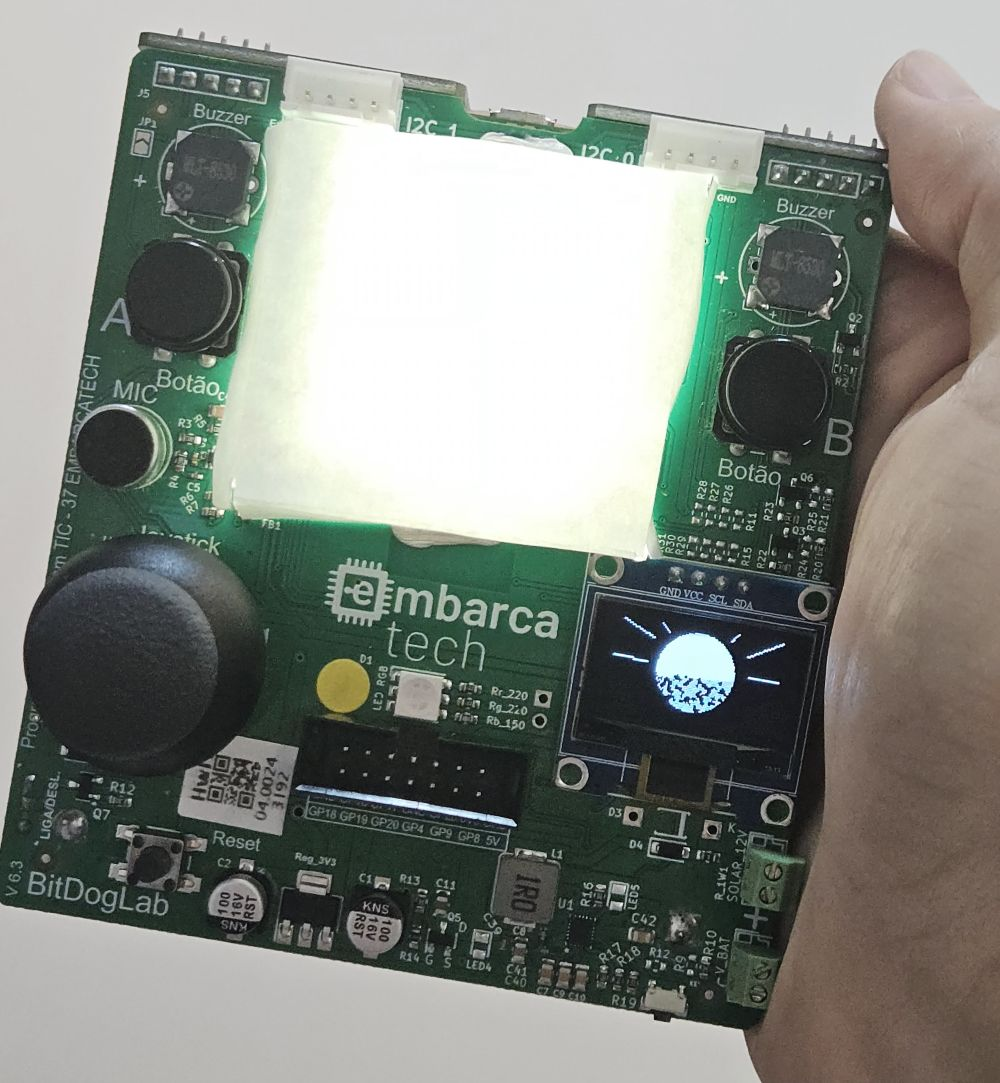
\includegraphics[width=0.3\textwidth]{resources/profilepicture.jpg}
    \caption{Janela de Pixels(Sol)}
    \label{fig:profilepicture}
\end{wrapfigure}

Após obtida a rede WiFi, o código atualizará o relógio interno do Raspberry Pi Pico usando um servidor NTP e, se, por algum motivo não for possível obter um horário o código automaticamente definirá um horário padrão(12:00). Após feito isso, a matriz de LEDs será ligada automaticamente e começará a pulsar com as cores pré-definidas de acordo com o horário. O display também será ligado e mostrará um desenho de acordo com o especificado.
A partir daí os botões A ou B da placa BitDogLab poderão ser pressionados para desligar o display e matriz de LEDs.

\subsection{Justificativa}
Como concluído por CANAZEI et al. (2017)\cite{canazeietal} existe uma correlação entre a presença de clarabóias artificiais e a redução de sentimentos negativos, demonstrando a necessidade de projetos nessa linha de pesquisa. A Janela de Pixels é um exemplo de como a tecnologia pode ser usada para melhorar o bem-estar em ambientes fechados. Através da simulação das cores do céu, o projeto busca trazer um pouco do mundo exterior para dentro de ambientes sem janelas, proporcionando uma experiência mais agradável e menos estressante para os usuários.

\subsection{Originalidade}
\begin{wrapfigure}{R}{0.3\textwidth}
    \centering
    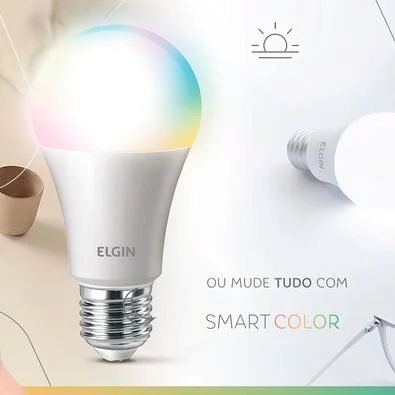
\includegraphics[width=0.25\textwidth]{resources/lampadasmart.jpg}
    \caption{Lâmpada Smart.}
    \label{fig:lampadasmart}
\end{wrapfigure}
Um dos requerimentos definidos pelo curso de capacitação é a originalidade, para isso foram feitas pesquisas de produtos similares já existentes no mercado. Vários produtos foram encontrados, como a clarabóia artificial mencionada em (2017)\cite{canazeietal}, no entanto o produto que mais se aproxima da Janela de Pixels em preço, tamanho e escopo são as \textbf{Lâmpadas Smart}. Existem dezenas de opções no mercado, com uma ampla gama de preços. As funções são extremamente parecidas: brilhar com cores diferentes durante o dia, com esquemas de cores escolhidos pelo usuário. A partir daí levanta-se uma dúvida: 

O que a Janela de Pixels trás de novo?

Produtos similares comumente apresentam software fechado impossibilitando qualquer tipo de auditoria independente ou modificação. Dessa forma, as possibilidades de customização são extremamente limitadas, quando não completamente inexistentes, restringindo a experiência do usuário às configurações predefinidas pelo fabricante. Além disso, há ainda a preocupação crescente com os riscos à privacidade, já que a grande maioria desses produtos exige uma conexão contínua com um aplicativo próprio, que frequentemente solicita permissões excessivas e desnecessárias para seu funcionamento adequado.

Nesse quesito, a Janela de Pixels se destaca por seu software totalmente aberto e disponível no GitHub, permitindo auditoria para garantir transparência e confiança. Seu funcionamento simples e eficiente evita a coleta indevida de dados, oferecendo mais segurança e respeito à privacidade dos usuários. Assim, a Janela de Pixels se torna uma alternativa diferenciada, priorizando funcionalidade, liberdade e segurança.

\paragraph{}Além disso, pode-se olhar para o projeto de um ângulo \textit{faça você mesmo}(DIY). Nessa área o leque de projetos disponíveis aumenta substancialmente. Uma busca rápida revelou vários exemplos distintos de projetos que tentam resolver o mesmo problema, no entanto nenhum é exatamente igual em termos de facilidade de uso e implementação:

\begin{figure}[H]
    \centering
    \begin{subfigure}[t]{.3\textwidth}
      \centering
      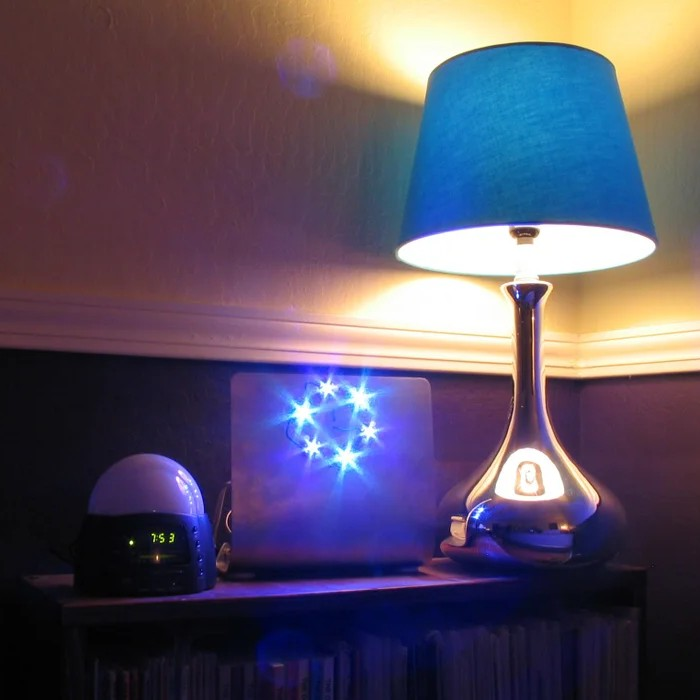
\includegraphics[width=.9\linewidth]{resources/example1.jpg}
      \caption{\href{https://www.instructables.com/Arduino-Controlled-Sunrise-Alarm-Clock/}{Sunrise Alarm Clock}}
    \end{subfigure}%
    \begin{subfigure}[t]{.3\textwidth}
      \centering
      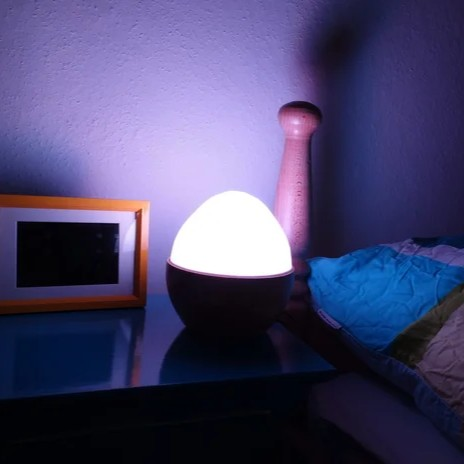
\includegraphics[width=.9\linewidth]{resources/example2.jpg}
      \caption{\href{https://www.instructables.com/WeggUp-A-sleeping-cycle-and-light-alarm-clocke/}{Sleeping Cycle and Light Alarm}}
    \end{subfigure}
    \begin{subfigure}[t]{.3\textwidth}
        \centering
        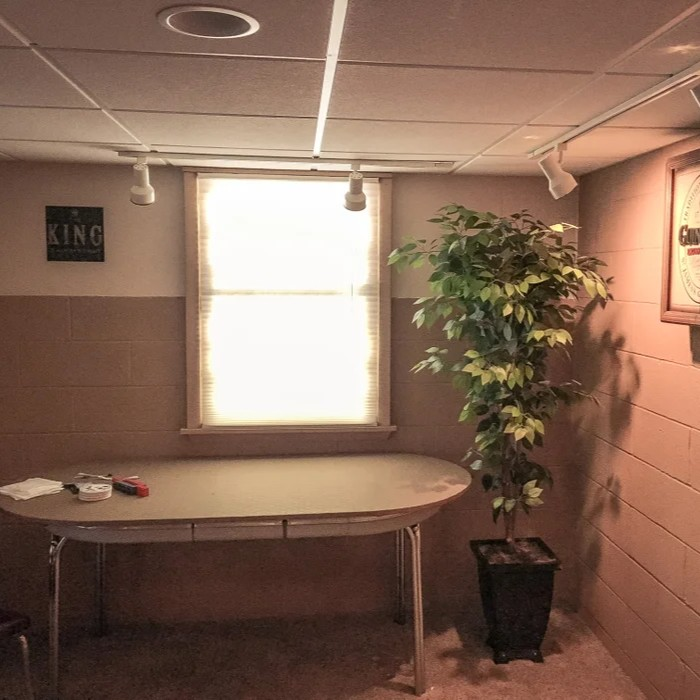
\includegraphics[width=.9\linewidth]{resources/example3.jpg}
        \caption{\href{https://www.instructables.com/Smart-LED-Window/}{Smart LED Window}}
      \end{subfigure}
    \caption{Exemplos de projetos similares}
    \label{fig:Projetos_Similares}
\end{figure}

No entanto todos esse projetos tem como característica definitiva seu hardware implementado do zero. Todos eles usam microcontroladores como o Arduino e manualmente conectam os componentes peça a peça, o que reduz sua confiabilidade e aumenta substancialmente o conhecimento requerido para implementar sua própria versão. Nesse ângulo o requerimento de uso da BitDogLab simplifica a implementação de versões próprias para os usuários, pois não existe necessidade de implementar cirucitos do zero. Na BitDogLab todos os componentes são preconectados e basta apenas gravar o software necessário para ter sua própria versão da Janela de Pixels.

Em termos técnicos a maioria dos projetos DIY também usam plataformas mais antigas como Arduinos e ESP32. Logo a Janela de Pixels mostra-se inovadora com o uso de uma MCU recente na forma do RP2040.
\section{O Hardware}
\subsection{Diagrama de Blocos}
\begin{figure}[H]
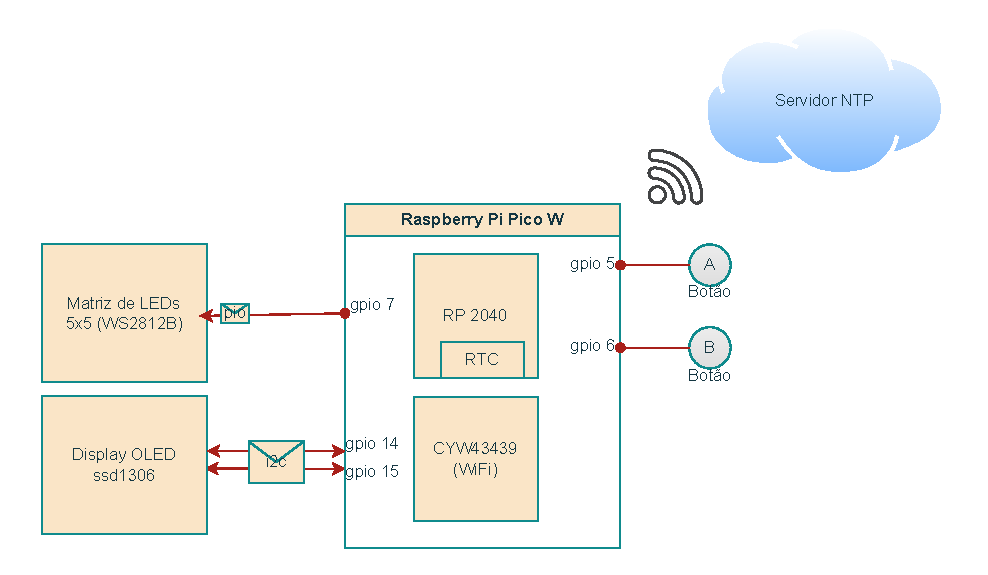
\includegraphics{resources/diagramablocos.pdf}
\caption{Diagrama de blocos demonstrando o hardware} 
\end{figure}
\begin{wrapfigure}{R}{0.4\textwidth}
    \centering
    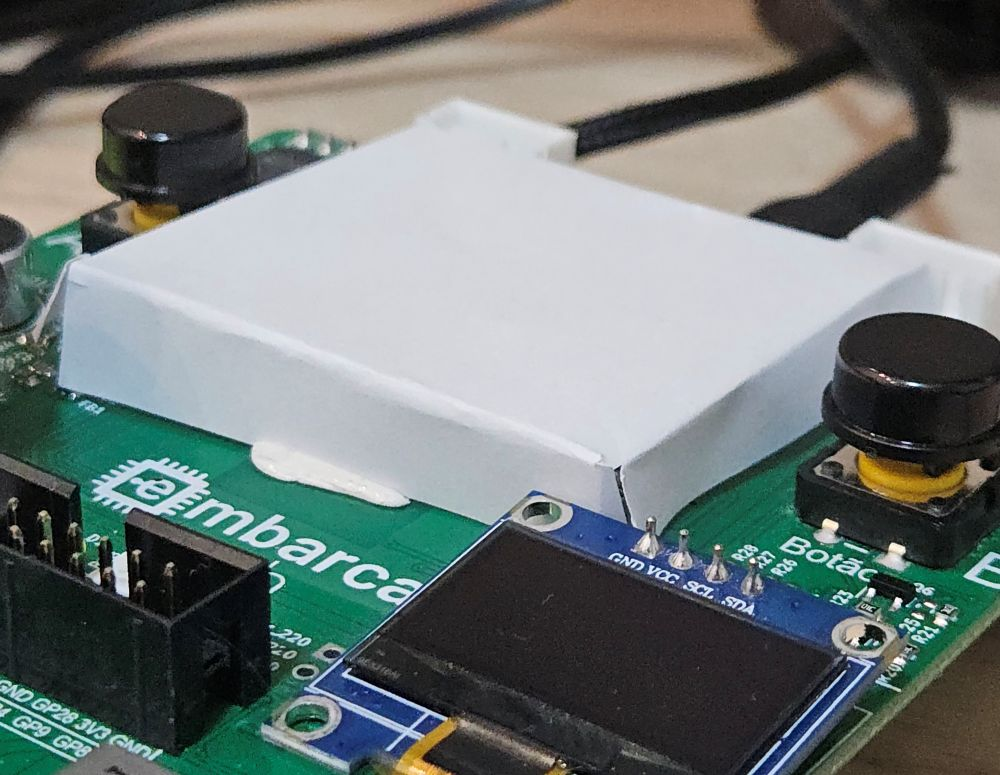
\includegraphics[width=0.35\textwidth]{resources/difusor.jpg}
    \caption{Difusor de papel sulfite.}
    \vspace{-30pt}
    \label{fig:difusor}
\end{wrapfigure}
\subsection{Função de cada bloco}

\paragraph{Matriz de LEDs 5x5}

Pulsa com as cores escolhidas nas definições do cliente. Mudando de acordo com o horário. Um pequeno difusor feito de papel sulfite foi adicionado em cima da matriz de LEDs para suavizar as cores. Note que o objetivo do difusor não é reduzir a luminância, mas sim uniformizar a cor.

\paragraph{Display OLED 128x64 ssd1306}
Exibe imagens de acordo com as definições do cliente. Mudando de acordo com o horário. Também serve para mostrar mensagens informativas ao usuário como o status da conexão do WiFi e atualização do horário. 

\paragraph{RP 2040 -> RTC}
O periférico digital \textit{real time clock}(RTC) do RP2040 é utilizado como o relógio do projeto.

\paragraph{CYW43439 -> WiFi}
O chip se conecta ao WiFi e entra em contato com um servidor de \textit{Network Time Protocol}(NTP) o horário recebido é guardado no RTC.

\paragraph{Botões A e B}
São simplesmente utilizados para ligar e desligar o display e a matriz de LEDs

\subsection{Configuração de Cada bloco}

\paragraph{Matriz de LEDs 5x5}
A matriz de 25 LEDs WB2812B, conectada no modo cascata, é controlada primariamente por software, o módulo PIO é utilizado para gerar o protocolo necessário para a comunicação. A linha DIN da matriz está conectada na GPIO 7 do Pico

\paragraph{Display OLED 128x64 ssd1306}
Os pinos SDA e SCL do OLED estão conectados nas GPIO 14 e 15 respectivamente. O endereço I2C é 0x3c com um clock speed 400khz.

\paragraph{RP 2040 -> RTC}
O horário guardado pelo RTC é definido pelos dados recebidos do servidor NTP.

\paragraph{CYW43439 -> WiFi}
O módulo WiFi está configurado para funcionar no modo estação para poder estabelecer conexões com redes WiFis já existentes. Ou seja é o modo cliente do WiFi.

\paragraph{Botões A e B}
Os botões estáo conectados nas GPIOs 5 e 6 respectivamente e são configurados com resistores de pull up.

\subsection{Especificações}

O hardware descrito atende as especificações dos clientes de forma eficiente e prática. A matriz de LEDs 5x5, controlada pelo RP2040, exibe cores que mudam de acordo com o horário do dia, proporcionando uma representação visual do céu externo. O uso do difusor de papel sulfite sobre a matriz de LEDs garante que as cores sejam uniformes e agradáveis aos olhos, sem mudanças bruscas de luminosidade que poderiam distrair os usuários. Além disso, a matriz de LEDs desliga automaticamente durante o período noturno, economizando energia e evitando qualquer perturbação durante o sono.

O display OLED 128x64 ssd1306 complementa a matriz de LEDs ao exibir imagens representativas do período do dia, como sol, lua e estrelas, conforme especificado pelos clientes. A conectividade WiFi, proporcionada pelo chip CYW43439, permite que o dispositivo obtenha o horário atual de um servidor NTP, garantindo que as cores e imagens exibidas estejam sempre sincronizadas com o horário real. Os botões A e B oferecem uma interface simples para ligar e desligar o display e a matriz de LEDs, atendendo ao requisito de facilidade de uso e configuração mínima.

\subsection{Lista de Materiais}
Os únicos materias externos à placa de desenvolvimento é o pequeno quadrado de papel sulfite utilizado como difusor. No entanto caso seja necessária a implementação usando componentes discretos a lista de materias é a seguinte:
\begin{itemize}
    \item 1x Microcontrolador Raspberry Pi Pico W
    \item 25x LEDs WB2812B
    \item 1x Display OLED 128x64 ssd1306
    \item 1x Botão de pressão
    \item 1x Difusor de papel sulfite
\end{itemize}

\subsection{Descrição da Pinagem Usada}

\begin{table}[H]
    \centering
    \begin{tabular}{|c|c|c|c|}
        \hline
        \textbf{Componente} & \textbf{Descrição} & \textbf{GPIO} & \textbf{Pico W Pin} \\
        \hline
        Matriz de LEDs 5x5 & Data In (DIN) & GPIO 7 & Pin 10 \\
        \hline
        Display OLED 128x64 & SDA & GPIO 14 & Pin 19 \\
        \hline
        Display OLED 128x64 & SCL & GPIO 15 & Pin 20 \\
        \hline
        Botão A & Input & GPIO 5 & Pin 7 \\
        \hline
        Botão B & Input & GPIO 6 & Pin 9 \\
        \hline
    \end{tabular}
    \caption{Pinagem dos Componentes}
    \label{tab:pinagem}
\end{table}
\subsection{Circuito Completo}
\begin{figure}[H]
    \centering
    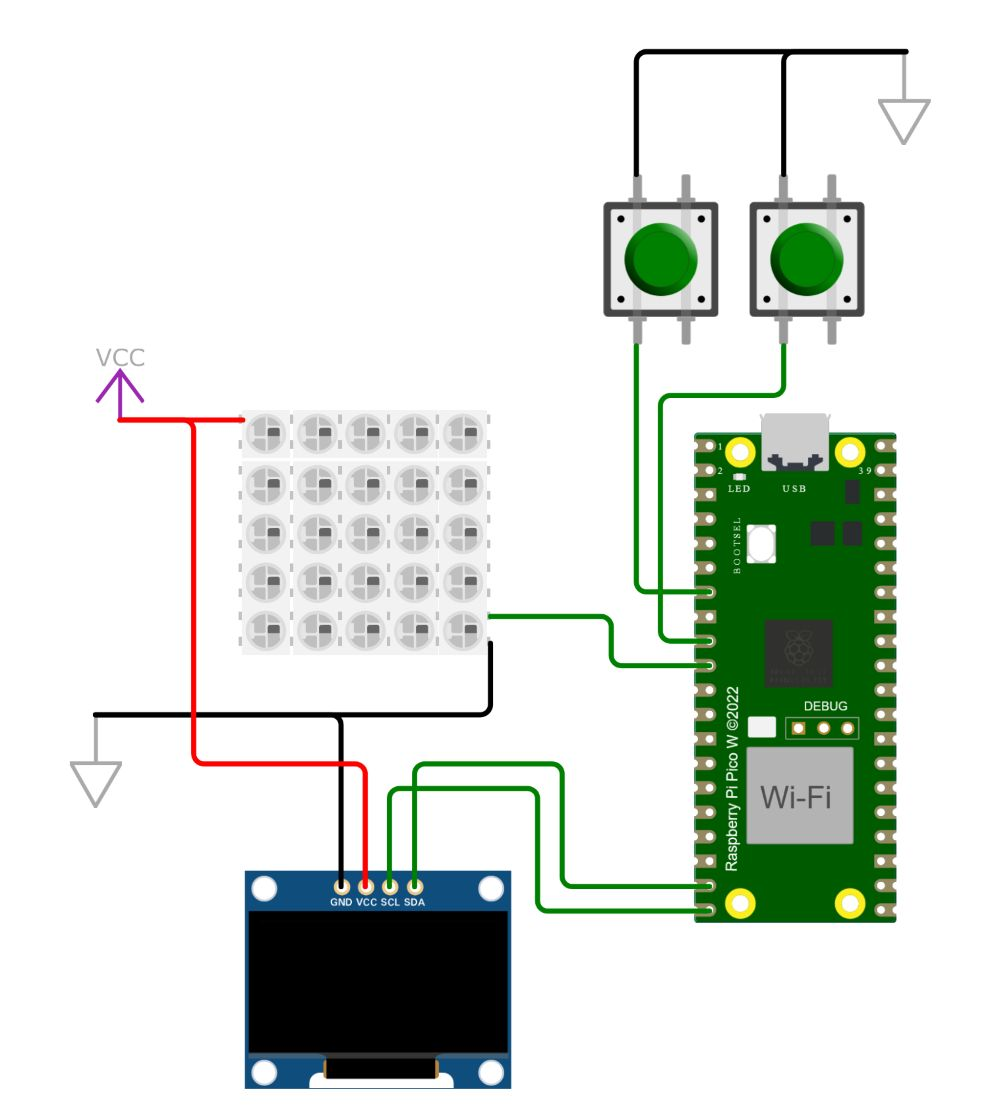
\includegraphics[width=0.5\textwidth]{resources/diagram.jpg}
    \caption{Diagrama do Circuito}
    \vspace{-40pt}
    \label{fig:diagram}
\end{figure}


\section{O Software}

\subsection{Blocos funcionais}
\begin{figure}[H]    
    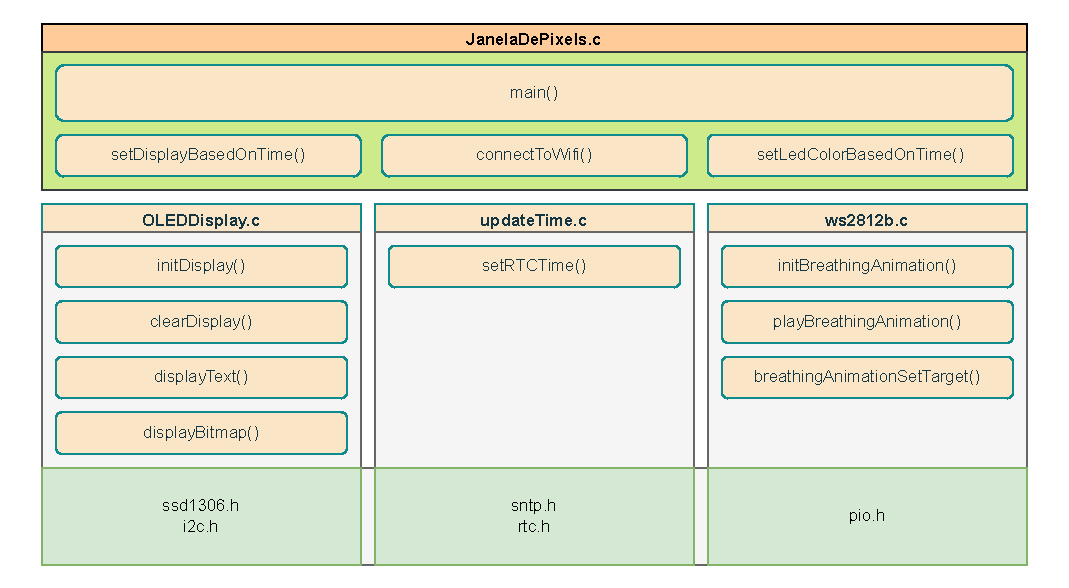
\includegraphics[width=0.99\textwidth]{resources/blocklayers.pdf}
\end{figure}

\subsection{Funcionalidades}
O programa apresenta uma separação classica em 3 camadas distintas:
\begin{enumerate}
    \item Aplicação
    \item Serviço
    \item Abstração de Hardware 
\end{enumerate}
Na camada de aplicação temos a função main que inicializa os diversos pinos, e orquestra as chamadas para outras funções de alto nível, que mudam a cor e as imagens mostradas na matriz de LED e no display, além de conectar a uma rede WiFi e chamar a função para conectar ao relógio.

Logo em seguida temos a camada de serviço:
\paragraph{OLEDDisplay.c} Responsável por atualizar o display com os dados providenciados pelas funções de alto nível. Baseado nos exemplos do repositório BitDogLabC \cite{BitDogLabC}
\paragraph{updateTime.c} Contém as funçoes de conexão a um servidor NTP e atualização do relógio interno.
\paragraph{ws2812b.c} É responsável pela constante animação da matriz de LEDs e inicialização da função de PIO que gera os sinais necessários para controlar a matriz, foram usados como base exemplos encontrados na internet \cite{HelloPIO} e nos exemplos oficias da Raspberry Pi \cite{picoexamples} 

E por fim a camada de abstração de hardware, nessa camada foram usadas somente bibliotecas já existentes.
\paragraph{ssd1306.h} Responsável pelo display OLED. \cite{BitDogLabC}
\paragraph{i2c.h} Implementa o protocolo de comunicação utilisado pelo display
\paragraph{sntp.h} SimpleNTP: Estabelece a conexão com um servidor NTP usando uma api simplificada. Ver a documentação em \cite{sntp}
\paragraph{rtc.h} Responsável pelo relógio interno do RP2040
\paragraph{pio.h} É utilizado para o controle direto e preciso da matriz de LED
\pagebreak
\subsection{Definição das variáveis}
\paragraph{main.c: bool isAnimationPlaying} Verdadeiro se a animação deve rodar. Falso caso contrário. Seu estado muda quando o usuário pressiona um botão.
\paragraph{main.c: TimeColorMapping\ color\_map[]} Array do tipo TimeColorMapping, contém o mapeamento entre as horas do dia e as cores definidas pelos clientes.
\paragraph{main.c: breathing\_animation\_state\_t anim} Estrutura que contém os dados da animação sendo rodada na matriz de LEDs.

\paragraph{updateTime.c: int sntp\_time\_updated} 1 se o servidor NTP retornou um horário valido. 0 se não. 
\paragraph{updateTime.c: time\_t ntp\_time} Horário retornado pelo servido NTP.

\paragraph{ws2812b.c: uint8\_t brightness} definida como \((\exp(\sin(millis / 2000.0 \times \pi)) + 0.815) \times 22.639\) essa é a variável chave para o funcionamento do efeito de respiração da matriz de leds. Baseado no trabalho de STÖR\cite{thingpulse}

\paragraph{moon.h: moon\_bits[]} Array de bytes que representa a imagem da Lua.
\paragraph{stars.h: star\_bits[]} Array de bytes que representa a imagem das estrelas.
\paragraph{sun.h: sun\_bits[]} Array de bytes que representa a imagem do sol.

\begin{figure}[H]
    
\includegraphics[width=0.33\textwidth]{resources/sun.png}
    
\includegraphics[width=0.33\textwidth]{resources/moon.png}
    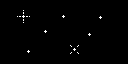
\includegraphics[width=0.33\textwidth]{resources/stars.png}
    \caption{Bitmaps mostrados no display}
\end{figure}

\subsection{Fluxograma}

\begin{figure}[H]
    \center
    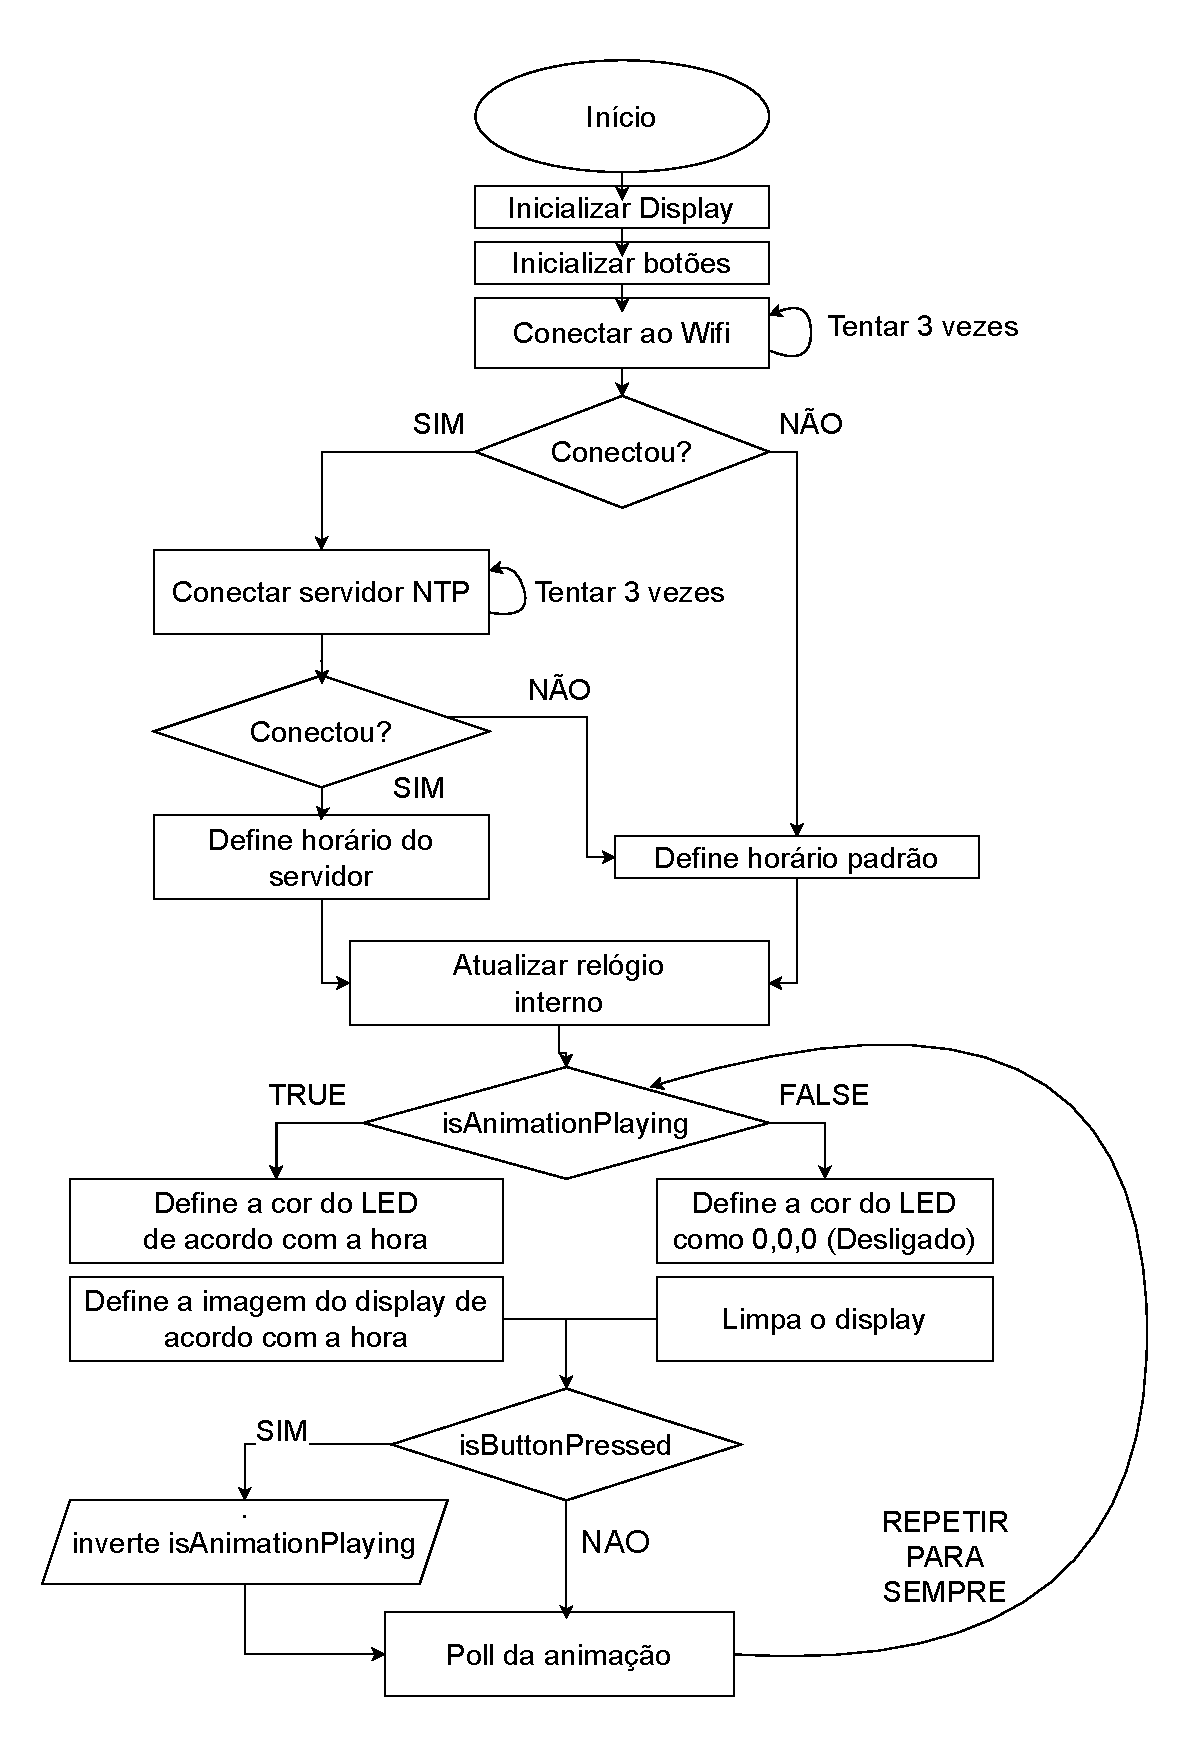
\includegraphics[width=0.78\textwidth]{resources/softwareflowchart.pdf}
    \caption{Fluxograma do software} 
    \vspace{-40pt}
\end{figure}
\pagebreak
\subsection{Inicialização}
\paragraph{Display} Inicializado com os pinos no modo pull up. O clock I2C é definido como 400 kHz.
\paragraph{Inicializar botões} As GPIOs nas quais os botões estão conectados é são definidos como input e colocadas no modo pull up.
\paragraph{WiFi} O chip de WiFi é colocado no modo station.
\paragraph{RTC} O real time clock é inicializado com um horário, advindo de um servidor NTP em caso de sucesso, ou pré-definido em caso de problemas.
\paragraph{ws2812b} É adquirida uma máquina PIO livre que é então carregada com um programa responsável por gerar os sinais de controle dos LEDs neopixel.

\subsection{Configuração dos registros}
\paragraph{JanelaDePixels.c: TimeColorMapping} Mapeia um horário para uma cor RGB específica, os valores iniciais são as cores definidas pelos clientes.
\paragraph{ws2812b.c: breathing\_animation\_state\_t} Guarda as principais informações sobre o estado da animação pulsante dos LEDs, como:
\begin{enumerate}
    \item Endereço da máquina PIO na qual o protocolo de comunicação será enviado. Obtido na inicialização.
    \item Alvo da cor para a animação {RGB 8bpc}. Atualizado frequentemente pelo laço principal
    \item Cor atual, depois de ser modulada pela equação da animação. {RGB 8bpc}. Atualizado no loop de polling da animação
    \item Tempo restante até a próxima atualização da animação. (em ms) Atualizado no loop de polling da animação
    \item Intervalo esperado entre as atualizações (em ms) Atualizado no loop de polling da animação
\end{enumerate}
\paragraph{OLEDDisplay.c: render\_area} Guarda as dimensões da área disponível para desenhar no display 128x64. Inicializado para 0, 127 e 0, 63

\subsection{Estrutura e formato de dados} Os dois principais tipos de dados nesse projeto são a estrutura do mapeamento de cores e os bitmaps mostrados no display.
\paragraph{Mapeamento de cores para horários} O mapeamento é um struct bem básico: uint\_8t para o início e o fim do intervalo de horas. E 3 uint8\_t para as cores naquele intervalo: r, g, b.
\paragraph{Bitmaps:} O display ss1306 é monocromático portanto cada pixel só precisa de uma cor (1 bit per pixel), a memória do display é formada por páginas de 8 bits que representam uma linha inteira de 8 pixels. Logo para facilitar o carregamento de dados na memória do display os dados do bitmap são separados em págines de um byte, para representar uma imagem completa serão necessários 128x64 / 8 bits, ou seja 1024 bytes. A array que guarda o bmp tem exatamente 1024 entradas de um byte. Os bitmaps foram desenhados no GIMP e convertidos usando a ferramenta image2cpp\cite{Bitmapconverter}

\subsection{Organização da memória}
São usados ponteiros para passar valores entre as diferentes funções. Esses dados são alocados na stack de memória do Pico.
\subsection{Protocolo de comunicação}
\paragraph{WS2812B} Os LEDs são controlados por meio de um protocolo serial fio único. Uma máquina PIO é utilisada para gerar os sinais necessários de acordo com a datasheet dos LEDs:
Para sinal lógico 0 a saída é 3 ciclos HIGH e 7 ciclos LOW
Para sinal lógico 1 a saída é 6 ciclos HIGH e 4 ciclos LOW
Com um clock de 800khz as saídas geradas tem a duração esperada pelo chips dos LEDs como delineado no datasheet \cite{WS2812Bdatasheet}
\paragraph{ssd1306} Usa o protocolo i2c com um endereço 0x3c e um clock de 400 kHz.

\subsection{Formato de pacote de dados}
\paragraph{WS2812B} O pacote de dados esperado é uma sequencia de 24 bits no formato GRB, com 8 bits por pixel. Para formar esses dados são utilizados 3 variáveis do tipo uint8\_t e que são organizadas com operações shift, colocando-as em ordem começando pelos bits mais significativos. Então é aplicada uma operação OR entre as variáveis retornando um valor de 32 bits que é colocado no FIFO da máquina PIO, os ultimos 8 bits menos significativos são ignorados já que a máquina pio está programada para enviar apenas os 24 bits menos significativos.
\paragraph{SSD1306} O pacote de dados do OLED é composta de 1024 bytes, onde cada pixel é representado por um bit. O pacote é então enviado via I2C ao display.

\section{Execução}

\subsection{Metodologia}
\subsubsection{Ideação}
A parte mais difícil em um projeto conectado a um curso: a escolha de um problema a ser resolvido é uma parte essencial do processo. O problema deve ser resolvível no tempo permitido, levando em consideração os requisitos do curso em si (\ref{requisitoscurso}). Depois de escolhido o problema, um processo iterativo foi aplicado para definir e refinar a solução.
\subsubsection{Iteração} 
O método utilizado no projeto segue em grande parte o método iterativo híbrido apresentado por Cugnasca\cite{cugnasca}. Primeiramente é construída uma representação abstrata de um problema real, uma solução é então concebida no campo do pensamento, que por conseguinte é realizada no mundo real. Por meio de testes da solução o problema é redefinido e refinado, recomeçando o processo. Isso continua até que uma solução satisfatória seja encontrada.

A problema original deste projeto era a falta que os clientes sentem de serem acordados \textbf{naturalmente} pela iluminação solar. A solução original era simplesmente um alarme de luz. Depois de uma primeira tentativa de implementação aprendeu-se o suficiente sobre a natureza do problema e do hardware utilizado, percebeu-se que o escopo do projeto poderia ser aumentado para um tipo de relógio. Neste momento foram realizadas pesquisas sobre projetos parecidos, a fim de garantir um nível mínimo de originalidade do projeto. Como nenhum projeto idêntico foi encontrado a decisão de continuar com o processo de refinamento foi óbvia. Assim, depois de algumas iterações o resultado final foi alcançado.
\subsubsection{O Processo de Implementação}
O processo de implementação do projeto, ou seja, a fase de realização discutida por Cugnasca\cite{cugnasca} foi a fase que mais consumiu tempo. Aqui estão esboçadas a principais etapas:
\paragraph{Ambiente de desenvolvimento} A \textbf{IDE} de escolha foi o VSCode devido a sua compatibilidade ampla com o kit de desenvolvimento da Raspberry Pi Pico. Bastou apenas instalar as extensões necessárias para que o ambiente de desenvolvimento estivesse completamente funcional na minha máquina rodando WIndows 11.
\paragraph{Pesquisa} Entender o hardware é essencial para um projeto bem implementado. Aqui foram feitas pesquisas sobre o funcionamento e conexão do hardware da BitDogLab, nesse passo foram encontrados os datashets dos diversos componentes da placa. Os links estão na referência\cite{picosdkdocs} \cite{WS2812Bdatasheet}. Nessa etapa o documento mais útil foi o Banco de Dados de Hardware da BitDogLab\cite{BitDogLabBIH}. Também foram encontrados repositórios com exemplos de código. \cite{BitDogLabC} \cite{picoexamples}
Nessa etapa também fora utilizadas varias ferramentas de \textbf{LLM} para ajudar a filtrar as grandes quantidades de informações presentes nos datasheets e nos exemplos.
\paragraph{Código} Com um ambiente configurado e com os resultados das pesquisas em mãos foi possível começar a escrever o código necessário com confiança. Foi considerada a aquisição de uma segunda placa Raspberry Pi Pico para ser utilizada como debug probe, no entanto o risco de soldar os pinos necessários na BitDogLab se mostrou muito alto, logo foi necessário usar um método alternativo de \textbf{debbuging}: a função \textit{printf} da biblioteca textit{stdio} e o \textit{display OLED}. 
A primeira parte implementada do projeto foi, portanto, o código para mostrar texto no display, que assim serviria para mostrar mensagens de erro durante o desenvolvimento.

Após isso o código de conexão ao WiFi e subsequente conexão a um servidor NTP foi implementado. Nessa etapa fram adicionadas funções robustas que falham graciosamente se a conexão não acontecer com sucesso.
Por final o código de iluminação da matriz de LED foi implementado. Animações diferentes para a iluminação foram testadas, até a animação de respiração \cite{thingpulse} ser encontrada Durante a fase de testes dessa etapa foi encontrada a solução do difusor para uniformizar a luz da matriz de LEDs. 
Por fim os botões foram implementados para desligar os displays.

Aqui foi decidido que não haveria tempo o suficiente para cumprir os requisitos adicionais de exibição das condições climática no display. Consulte a seção \ref{requisitos}.

\subsection{Testes de Validação}

Para garantir que o projeto atenda aos requisitos especificados (\ref{requisitos}) e funcione corretamente, foram realizados diversos testes de validação. Esses testes foram executados ao mesmo tempo em que o código foi escrito para verificar o funcionamento de cada subsistema.

\subsubsection{Teste do Display OLED}
O primeiro teste foi a validação do texto exibido no display OLED.
\begin{enumerate}
    \item Definir um texto de teste no código.
    \item Verificar se o display OLED exibe o texto correto.
\end{enumerate}

\subsubsection{Teste de Conectividade WiFi}
A seguir foi necessário validar a conexão com o Wifi e a atualização do horário. O teste foi realizado da seguinte forma:
\begin{enumerate}
    \item Configurar um hotspot WiFi com as credenciais esperadas pela placa.
    \item Ligar a placa e verificar se a conexão WiFi foi estabelecida com sucesso.
    \item Verificar se o horário foi atualizado corretamente no display OLED.
\end{enumerate}

\subsubsection{Teste de Animação da Matriz de LEDs}
Depois veio a validação da animação de respiração da matriz de LEDs. O objetivo era garantir que os LEDs pulsassem com as cores corretas de acordo com o horário do dia:
\begin{enumerate}
    \item Configurar o horário manualmente para diferentes períodos do dia.
    \item Verificar se a matriz de LEDs exibe as cores corretas e se a animação de respiração está funcionando.
\end{enumerate}
Foi aqui que foi descoberta a necessidade do difusor.

\subsubsection{Teste do Display OLED 2}
O terceiro teste foi a validação das imagens exibidas no display OLED. O objetivo era garantir que as imagens corretas fossem exibidas de acordo com o horário do dia. O teste foi o seguinte:
\begin{enumerate}
    \item Configurar o horário manualmente para diferentes períodos do dia.
    \item Verificar se o display OLED exibe as imagens corretas (sol, lua, estrelas).
\end{enumerate}

\subsubsection{Teste dos Botões de Controle}
O quarto teste foi a validação dos botões de controle. O objetivo era garantir que os botões A e B pudessem ligar e desligar a matriz de LEDs e o display OLED. O teste foi realizado da seguinte forma:
\begin{enumerate}
    \item Pressionar individualmente os botões A e B. Verificou-se se a matriz de LEDs e o display OLED mudam de estado.
\end{enumerate}

\subsubsection{Teste Geral}
O último teste foi a validação do desempenho geral do sistema. O objetivo era garantir que todas as funcionalidades funcionassem corretamente em conjunto. O teste foi realizado da seguinte forma:
\begin{enumerate}
    \item Ligar a placa e verificar se todas as funcionalidades (conectividade WiFi, animação da matriz de LEDs, exibição de imagens no display OLED, controle dos botões) funcionam corretamente.
\end{enumerate}
O teste foi considerado bem-sucedido quando todas as funcionalidades funcionaram conforme esperado, sem erros ou falhas.

\subsection{Discussão dos resultados}
\subsubsection{Conclusão}
Os resultados obtidos com a implementação do projeto Janela de Pixels foram satisfatórios e atenderam aos requisitos especificados pelos clientes. A matriz de LEDs 5x5 pulsou com as cores corretas de acordo com o horário do dia, proporcionando uma representação visual do céu externo. O display OLED exibiu as imagens corretas (sol, lua, estrelas) conforme esperado, e a conectividade WiFi permitiu a atualização precisa do horário através de um servidor NTP. Os requisitos opcionais não foram implementados mas existe uma base sólida para facilitar sua futura implementação.

Os testes de validação demonstraram que todas as funcionalidades do sistema funcionaram corretamente em conjunto, sem erros ou falhas. A animação de respiração dos LEDs foi implementada com sucesso, e o difusor de papel sulfite garantiu uma uniformidade agradável das cores. Os botões de controle permitiram ligar e desligar a matriz de LEDs e o display OLED de forma eficiente. Assim o projeto é considerado confiável e útil para os clientes.

Em conclusão, a Janela de Pixels é um projeto viável e eficaz para melhorar o bem-estar em ambientes fechados, proporcionando uma experiência visual agradável e menos estressante. A confiabilidade do hardware e a simplicidade de uso tornam o projeto uma solução prática e inovadora para simular a iluminação natural em espaços sem janelas.

\subsubsection{Possíveis Melhorias}
Caso seja possível obter mais tempo para melhorias do projeto, aqui estão algumas sugestões:
\begin{itemize}
    \item Implementação de uma interface de usuário para configuração da rede WiFi, simplificando ainda mais o processo de configuração.
    \item Implementação de uma interface para escolha da paleta de cores da matriz de LEDs.
    \item Desenvolvimento de animações alternativas para a matriz de LEDs.
\end{itemize}

\section{Links}
\paragraph{Github:} \url{https://github.com/igorsousa-santos/JaneladePixels}
\paragraph{Vídeo:} \url{https://youtu.be/7x5U3GYz7Rg }

\pagebreak

\bibliographystyle{abnt}
\bibliography{references}

\begin{thebibliography}{9}

    \bibitem{cugnasca}
    CUGNASCA, C. E.
    \textbf{Projetos de Sistemas Embarcados.} Departamento de Engenharia de Computação e Sistemas Digitais. 
    \textit{Escola Politécnica da USP}, Fev. 2018

    \bibitem{canazeietal}    
    CANAZEI, Markus; POHL, Wilfried; BLIEM, Harald R.; MARTINI, Markus; WEISS, Elisabeth M.
    \textbf{Artificial skylight effects in a windowless office environment.} Building and Environment, v. 124, p. 69-77, 2017. DOI: https://doi.org/10.1016/j.buildenv.2017.07.045. Disponível em: https://annas-archive.org/scidb/10.1016/j.buildenv.2017.07.045. Acesso em: 20 fev. 2025.

    \bibitem{thingpulse}
    STÖR, Marcel;
    \textbf{Breathing LEDs: Cracking the algorithm behind our breathing pattern.}
    Disponível em: \url{https://thingpulse.com/breathing-leds-cracking-the-algorithm-behind-our-breathing-pattern/}.
    Acesso em: 20 Fev. 2025.

    \bibitem{BitDogLabBIH}
    FRUETT, Fabiano;
    \textbf{Banco de Informações de Hardware (BIH) da BitDogLab.}
    Disponível em: \url{https://docs.google.com/document/d/13-68OqiU7ISE8U2KPRUXT2ISeBl3WPhXjGDFH52eWlU}

    \bibitem{Bitmapconverter}
    JAVL et al;
    \textbf{image2cpp: Bitmap Converter.}
    Disponível em: \url{https://javl.github.io/image2cpp/}

    \bibitem{picosdkdocs}
    THE RASPBERRY PI FOUNDATION;
    \textbf{Pico C SDK Documentation.}
    Disponível em: \url{https://www.raspberrypi.com/documentation/pico-sdk/}

    \bibitem{WS2812Bdatasheet}
    WORLDSEMI;
    \textbf{WS2812B Intelligent control led integrated light source.}
    Disponível em: \url{https://cdn-shop.adafruit.com/datasheets/WS2812B.pdf}

    \bibitem{BitDogLabC}
    \textbf{BitDogLab em C.}
    Disponível em: \url{https://github.com/BitDogLab/BitDogLab-C}

    \bibitem{HelloPIO}
    SHARMA, S. S.
    \textbf{Hello PIO.}
    Disponível em: \url{https://parthssharma.github.io/Pico/HelloPIO.html}

    \bibitem{RP2040DataSheet}
    THE RASPBERRY PI FOUNDATION;
    \textbf{RP2040 Datasheet}
    Disponível em: \url{https://datasheets.raspberrypi.com/rp2040/rp2040-datasheet.pdf}

    \bibitem{sntp}
    \textbf{lwip SNTP}
    Disponível em: \url{https://www.nongnu.org/lwip/2_0_x/group__sntp.html}

    \bibitem{picoexamples}
    \textbf{Raspberry Pi Pico C SDK Examples.}
    Disponível em: \url{https://github.com/raspberrypi/pico-examples/tree/master}

    \end{thebibliography}

\end{document}

\end{document}